\chapter{Price and value models}
In questo capitolo saranno mostrati alcuni dei fondamenti economici del Cloud computing. Molte tecnologie infatti vengono progettate in funzione del prezzo e dei modelli di vendita: ciò risulta necessario perché il prezzo rappresenta l'interfaccia verso l'utente. Il beneficio di un servizio deve giustificare il prezzo.

Ogni impresa, azione, prodotto, è soggetto ad un costo e ad un beneficio. Il costo di un cloud service spesso è il primo elemento che viene considerato, e i servizi vengono divisi in base ai modelli di prezzo (\textit{price models}).

\vspace{5mm}

I \textit{value models} invece sono quelli che il customer deve considerare per valutare in maniera quantitativa i benefici di cui godrà usufruendo di certi servizi.

\begin{mdframed}[backgroundcolor=gray!20,shadow=false]
\begin{itemize}
    \item I \textbf{price models} rispondono alla domanda \textit{"quanto costa?"} e sono definiti dal provider.
    \item I \textbf{value models} rispondono alla domanda \textit{"quanto beneficio mi dà?"} e sono misurati dal consumer.
\end{itemize}
\end{mdframed}

\begin{figure}[ht]
    \centering
    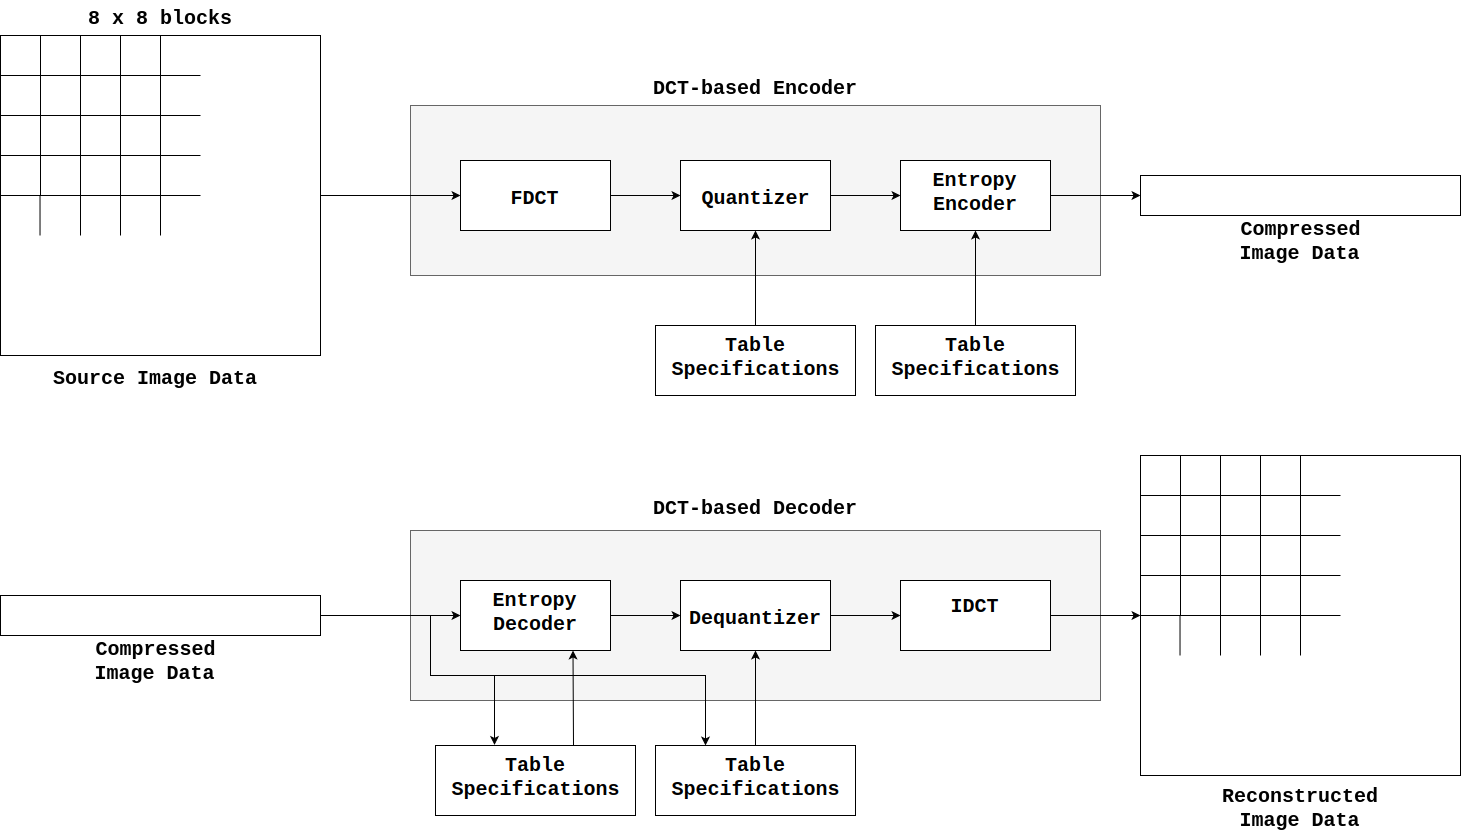
\includegraphics[width=7cm]{./Images/cap6/6.1.png}
\end{figure}

\section{Price models}
I price models permettono di stabilire il prezzo che un cliente è disposto a pagare per ricevere il valore di un prodotto o di un servizio. Un cloud service provider calcola questo prezzo considerando i costi operativi e di fornitura. Il modello di costo poi viene convertito in un price model. Tuttavia i price models non dipendono solo dal modello di costo, ma anche da altri fattori come il business model, le strategie di marketing, o dalle attese di guadagno e profitto.

Esempi chiari sono dati dai pionieri in alcune tecnologie, si pensi ad Apple con il primo telefono con touchscreen facile da usare, a Google con il primo motore di ricerca funzionale e Mark Zuckerberg con il primo social network mondiale.

\vspace{5mm}

Ogni modello di prezzo parte da un modello di costo, che comprende sia le spese in conto capitale che che quelle operative per la manutenzione e l'aggiornamento di un servizio. Normalmente infatti ogni 3-5 anni è necessario un cambio di tecnologie a causa di obsolescenza (hardware), oppure sicurezza, portabilità, efficienza (software).

Il \textit{cost model} include l'inflazione, le variazioni di cambio, la svalutazione, i costi di elettricità, licenze software e costo della manodopera. I modelli di prezzo si dividono in varie categorie (le prime due proprie del Cloud, le altre utilizzate anche da business innovativi):
\begin{itemize}
    \item Utility Price models
    \item Service Price models
    \item Performance Price models
    \item Marketing-oriented Price models
    \item Hybrid Price models
\end{itemize}

\subsection{Utility Price models}
Sono quelli che prevedono il monitoraggio dell'utilizzo della risorsa o del servizio da vendere. Il pagamento è in base al monitoraggio effettuato. Distinguiamo tre tipologie di Utility Price models:

\subsubsection{\textbf{CONSUMPTION-BASED}}
È il modello più usato per IaaS e PaaS, perché si integra perfettamente con il modello pay-per-use. Il prezzo viene fornito in base alla misurazione dell'utilizzo che il cliente fa del servizio, su base giornaliera, settimanale o mensile. Va molto bene per misurare risorse "grezze", come velocità del processore, GB trasferiti, memoria utilizzata, ecc. Per modelli come SaaS, INaaS o BPaaS è meno indicato: nel caso di INaaS ad esempio, dato un servizio che fornisce regole sulla tassazione, avrebbe poco senso calcolare la quantità di CPU utilizzata in quanto ci sono categorie di costi diversi.

\subsubsection{\textbf{TRANSACTION-BASED}}
È un modello business-related: il prezzo si basa su transazioni anziché sulla quantità di risorse consumate. Più evoluto rispetto al modello consumption-based ma può essere utilizzato anche per le modalità più grezze, usando ad esempio la larghezza di banda come indicatore di calcolo. Un modello consumption-based può infatti diventare transaction-based controllando la banda utilizzata per ogni transazione.

Dividendo il costo del servizio per un certo periodo si ottiene l'\textbf{Unit Transaction price}. Il modello transaction-based è utile se il volume delle transazioni è conosciuto o predicibile, oppure se il volume delle transazioni è legato ad alcuni fattori come ad esempio il numero di ore di lavoro. Molto adatto per INaaS e BPaaS, perché standardizza le transazioni, facendole diventare l'unità atomica del servizio offerto.

\subsubsection{\textbf{SUBSCRIPTION-BASED}}
Il prezzo del servizio è fisso e si paga periodicamente. A prescindere dall'utilizzo, il prezzo da pagare è sempre lo stesso. Può essere utilizzato per tutti i modelli di deployment. Netflix è un servizio subscription-based.

\subsection{Service Price models}
In questi modelli di prezzo non ci si riferisce più ad un consumo di risorse, bensì ai benefici che vengono dati in accordo ad un SLA. La differenza sta nel fatto che i servizi vengono offerti basandosi sulla QoS stabilita negli SLA. Distinguiamo tre modelli.

\subsubsection{FIXED}
Il prezzo (fisso) viene specificato su base mensile/annuale. Si può utilizzare se lo scopo è definito in maniera chiara ed è allineato con gli obiettivi a breve termine. Trasferisce i rischi nel senso che il consumer paga il provider per prendersi il rischio di gestire il servizio al posto suo. I rischi vengono misurati negli SLA e possono essere di vario tipo, come ad esempio che il costo possa essere più oneroso rispetto al pagamento pattuito.

\subsubsection{VOLUME-BASED}
Indica il volume di utenti, storage, transazioni, banda, ecc. Definisce in pratica il volume di un servizio, da misurare e da calcolare. Ovviamente anche qui cambia in base al business. Molto simile al subscription-based.

\subsubsection{TIERED}
Basato su Sla, su volume, o su un certo tipo di ammontare speso. Vengono definiti dei Tier, e a seconda del costo i servizi vengono offerti in modo diverso. È molto importante perché aggiunge valore al lavoro svolto, e soprattutto i clienti non sanno mai di cosa hanno bisogno quindi metterli davanti a più scelte spesso si rivela la strategia vincente. Questo modello può essere usato in tutti i modelli di deployment.

\begin{figure}[ht]
    \centering
    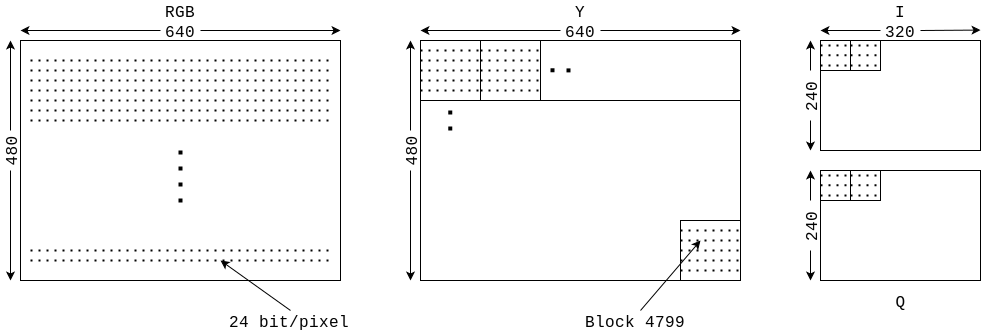
\includegraphics[width=8cm]{./Images/cap6/6.2.png}
\end{figure}

\subsection{Performance Price models}
Si basa sul fatto che esiste una soglia considerata per valutare e decidere il prezzo. Questa metrica è tipicamente legata al business goal del cliente, per cui richiede un output chiaro e definito, e allineato con il processo di business. Distinguiamo tre tipi: Outcome-based, Business-linked e Gain-share.

\subsubsection{OUTCOME-BASED}
Essenzialmente lega il pagamento "bonus" al cloud provider per un risultato che riduce il \textit{time to market} di un certo servizio (è legata quindi al valore percepito dal customer). Se si raggiunge un certo obiettivo di performance viene di solito assegnato un premio, e tipicamente viene usato insieme ad altri modelli, come ad esempio il fixed price.

\subsubsection{BUSINESS-LINKED}
Serve a collegare i contributi del cloud computing con alcuni indicatori di performance che influenzano il business model. Si può vedere chiaramente nel grafico seguente.

\begin{figure}[ht]
    \centering
    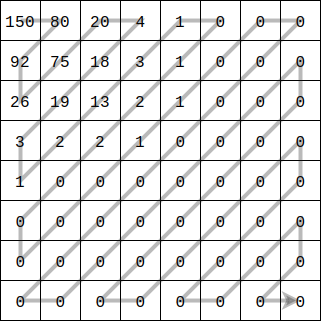
\includegraphics[width=6cm]{./Images/cap6/6.3.png}
\end{figure}

\subsubsection{GAIN-SHARE}
È un meccanismo abbastanza diffuso nelle startup per avere delle \textit{equity}, ovvero delle azioni dell'azienda. Il concetto è lavorare nella stessa direzione per favorire le acquisizioni delle azioni, ad esempio il service provider potrebbe essere premiato con una condivisione dei profitti del consumer se si raggiunge una certa quota. Anche questo può essere combinato con altri modelli.

\subsection{Marketing-oriented Price models}
A volte i price model vengono guidati dal marketing piuttosto che dalle prestazioni: i modelli osservati di seguito si impongono l'obiettivo di attrarre più clienti possibili, per poi monetizzare grazie a loro.

\subsubsection{FREEMIUM}
Il modello freemium ha due sottomodelli:
\begin{itemize}
    \item \textbf{try before buy}: di solito viene offerto un periodo di prova che permette di usufruire del servizio al 100\% senza pagare ma solo per una quantità di tempo stabilita, di solito 7 o 30 giorni.
    \item \textbf{pure freemium}: il servizio viene offerto gratuitamente ma spesso contiene annunci pubblicitari. È molto usato soprattutto nei modelli Saas (Dropbox, Linkedin). Offrono funzionalità limitate ma permettono un upgrade ad un servizio premium con feature aggiuntive.
\end{itemize}
L'idea di questo modello consiste nell'attirare una grande quantità di clienti per poi convincere una piccola quantità ad acquistare il servizio.

\subsubsection{RAZOR AND BLADES}
Come suggerisce il nome, si rifà proprio al mercato delle lamette usa e getta: che consiste nella vendita di una parte base (il rasoio) e di parti intercambiabili che vengono acquistate a cadenza temporale (le lamette). Basti pensare anche dalle stampanti a inchiostro o dalle macchinette del caffè. Alcuni esempi sono Amazon Alexa, Google Home o Amazon Kindle.

\subsection{Hybrid Price models}
Questi modelli consistono nel combinare diversi dei modelli visti in precedenza. Si rifanno tutti ad una strategia base, ovvero quella secondo la quale quando un utente entra in un ecosistema e si trova bene, diventa più facile indurlo a pagare per i servizi offerti, vedi Apple, Microsoft 365, ecc. I modelli ibridi si possono applicare a tutti i deployment models.


\section{Value models}
Indicano qual è il valore del servizio. Il valore è una qualità che viene percepita in base a ciò che rimane dopo che i benefici sono stati pesati. I benefici che l'utente riceve sono indicati nel SLA. Nel Cloud computing un model value è un pattern comune che definisce il valore per i customers. Distinguiamo sette modelli:
\begin{itemize}
    \item Operating expense;
    \item User demand flexibility;
    \item Price flexibility;
    \item Agility for time to market;
    \item Location flexibility;
    \item Asset optimization;
    \item Profit margin;
\end{itemize}

\vspace{5mm}
\begin{center}
    \texttt{cost} $\rightarrow$ \texttt{price} $\rightarrow$ \texttt{value} $\rightarrow$ \texttt{financial metrics}
\end{center}

\subsection{Operating expense}
Le spese del dipartimento IT dovrebbero essere all'inizio, per creare e mantenere il servizio, come d'altronde viene fatto con i SLA che sono stabiliti con il provider, i quali dettano la qualità del servizio che il dipartimento IT deve fornire. È importante che vengano considerate queste spese per gli investimenti che vengono fatti all'inizio in azienda, in quanto le spese per risorse IT sono sempre molto elevate. In due casi si verificano perdite nell'azienda: se la richiesta di capacity eccede la disponibilità del traditional computing oppure se si sta offrendo più capacità rispetto alle richieste.

\begin{figure}[htb!]
    \centering
    \includegraphics[width=7cm]{./Images/cap6/6.4.png}
\end{figure}

\subsection{User demand flexibility}
Ogni prodotto ha un proprio ciclo di vita, che in maniera astratta può essere sintetizzato in \textit{sviluppo, testing, lancio, marketing, gestione quotidiana}. In ciascuna di queste fasi ci sono differenti carichi di richieste, il che implica che bisogna gestire le richieste in modo differente, investendo o meno nella computing capacity, in quanto ad esempio durante il lancio del prodotto e le campagne di marketing sarà difficile adeguare le risorse in premise. Con il Cloud Computing inoltre l'audience di un prodotto è diventata globale, e la capacity deve flettersi in corrispondenza delle richieste durante il ciclo di vita del prodotto.

\begin{mdframed}[backgroundcolor=gray!20,shadow=false]
\textbf{Curiosità}: agli inizi dell'era di internet, le startup informatiche tremavano di fronte agli articoli tecnologici pubblicati dal giornale \textit{San Francisco Chronicles}. Spesso infatti accadeva che in seguito alla pubblicazione di un articolo su una certa startup, improvvisamente il carico di richieste aumentava vertiginosamente a causa dei lettori del giornale che volevano provare il servizio presentato, mandando nel panico i componenti della piccola impresa, che vedevano il loro sito andare down. Questo fenomeno è ancora conosciuto come \textit{Kiss of Death}.
\end{mdframed}

\begin{figure}[htb!]
    \centering
    \includegraphics[width=7cm]{./Images/cap6/6.5.png}
\end{figure}

\subsection{Price flexibility}
Con "prezzo" in questo modello intendiamo il prezzo del prodotto finale offerto dal consumer utilizzando i servizi del cloud provider. La price flexibility è chiara soprattutto nell'economia di scala: acquistando ad esempio 1000 server risparmierò sul prezzo unitario rispetto a se ne compro 5. Questo permette l'adozione di nuove tecnologie man mano che le vecchie raggiungono l'obsolescenza. Il valore che assume da parte del consumer è quello di poter contare su modelli di prezzo diversi che permettono di essere flessibile nell'offrire il servizio. Tipicamente i modelli tiered o quelli ibridi favoriscono la price flexibility.
\clearpage

\begin{figure}[hbt!]
    \centering
    \includegraphics[width=7cm]{./Images/cap6/6.6.png}
\end{figure}

\subsection{Agility for time to market}
Il \textit{time to market} è uno degli aspetti più importanti e il valore del cloud computing consiste nel fatto che diminuisce di tanto il tempo per lanciare il prodotto sul mercato. Questo è dovuto anche al fatto che è possibile switchare facilmente tra varie piattaforme, o fare il commissioning/decommissioning di componenti in maniera pressoché istantanea. È facile notare che nel traditional computing i tempi necessari per queste procedure ritardano l'arrivo del prodotto sul mercato.

\begin{figure}[hbt!]
    \centering
    \includegraphics[width=7cm]{./Images/cap6/6.7.png}
\end{figure}

\subsection{Location flexibility}
La possibilità di generare un mercato globale grazie al cloud computing viene raggiunta implicitamente senza dover richiedere un investimento separato e distinto. Con il traditional computing dovrei avere a disposizione diversi partner commerciali in giro per il mondo per il deploy del prodotto, mentre grazie al Cloud qualsiasi azienda ha già un potenziale mercato mondiale.
\clearpage
\begin{figure}[htb!]
    \centering
    \includegraphics[width=7cm]{./Images/cap6/6.8.png}
\end{figure}

\subsection{Asset optimization}
Questo modello ha come obiettivo l'ottimizzazione delle risorse fisiche dell'azienda. Uno degli aspetti da evitare infatti è la necessità di avere investimenti extra, per evitare perdita di affari o di reputazione. Anche l'ottimizzazione è importante quando ci si avvicina al termine del ciclo di vita del proprio servizio, in quanto è possibile terminare ad esempio un'istanza di un servizio in maniera brusca senza avere alcun problema dovuto al fatto che si hanno risorse inutilizzate.

\begin{figure}[htb!]
    \centering
    \includegraphics[width=7cm]{./Images/cap6/6.9.png}
\end{figure}

\subsection{Profit margin}
I margini di profitto sono importanti perché quando si produce un servizio i costi a valore aggiunto cadono ogni volta che l'esperienza o il valore raddoppia, ovvero le spese diminuiscono man mano che si produce esperienza\footnote{È stimato che con l'aumentare dell'esperienza i costi possano diminuire fino al 25\%.}. Un consumer affida le risorse IT della sua azienda ad un provider che gestisce molte situazioni e contesti simili, quindi può fare leva su un'esperienza molto ampia in modo da far diminuire i costi per il provider e anche per il consumer.
\clearpage
\begin{figure}[htb!]
    \centering
    \includegraphics[width=8cm]{./Images/cap6/6.10.png}
\end{figure}

\section{Financial metrics}
Le metriche finanziarie servono a fornire un valore effettivo ad un servizio cloud, utilizzando sia i price models che i value models. Possiamo distinguere quattro principali metriche finanziarie: payback method, net present value (NPV), return on investment (ROI), e time to market (TTM). Ce ne sono altre che possono essere utilizzate, come economic value added (EVA), return on assets (ROA), e return on equity (ROE). Tuttavia, queste metriche non sono adatte a servizi cloud ma vengono utilizzate principalmente per il settore business.

\subsection{Payback Method}
Misura il tempo necessario per recuperare un investimento per un prodotto o un servizio. Un servizio che ha un periodo di payback corto è meglio di uno che ha un periodo di payback lungo, come si può notare da questo esempio: supponiamo di acquistare un cloud service per \$1,000 al mese in modo da elaborare le fatture al doppio della velocità rispetto al sistema attuale di fatturazione. Considerando un anno, il prezzo è di \$12,000. Supponiamo ora che il vecchio sistema produce \$10,000 al mese di fatture, mentre il nuovo ne produce \$20,000. Il valore che cerchiamo è banalmente la differenza tra i due valori, quindi \$10,000. Considerando 30 giorni al mese, il guadagno giornaliero è di \$333. Ciò significa che il servizio cloud appena acquistato ci ripagherà (payback) dopo 36 giorni (12,000/333).

\vspace{5mm}

Generalmente il Payback Method viene utilizzato per le spese in conto capitale in quanto sono spese facili da analizzare e avvengono a monte di un progetto. Uno degli svantaggi di questo metodo è che non considera il tempo come valore, in quanto un bene posseduto ora ha valore maggiore dello stesso bene posseduto tra un anno, inoltre non tiene conto degli interessi. Per risolvere questo problema si utilizza il ROI.

\subsection{Return on Investment (ROI)}
Il ROI è utilizzatissimo nell'industria IT per gestire gli investimenti di capitale. La formula del ROI è la seguente:

\begin{center}
    $ROI = \frac{guadagno dell'investimento - costo dell'investimento}{costo dell'investimento}$
\end{center}

Prendiamo come esempio lo stesso cloud service di prima che costa \$1,000 al mese. Il ROI si calcola come segue: il guadagno dell'investimento come abbiamo detto è \$10,000 al mese, mentre il costo dell'investimento è \$1,000 al mese.
\begin{center}
    $ROI = \frac{\$10,000 - \$1,000}{\$1,000} = 900\%$
\end{center}
Per ottenere un valore più realistico del ROI si utilizza il NPV.

\subsection{Net Present Value (NPV)}
Quando sono presenti regolarmente più flussi di cassa dello stesso ammontare, questi si traducono in rendite per un'azienda. A causa degli effetti dell'inflazione e degli interessi nel tempo, un flusso di cassa di \$1,000 il mese prossimo vale di più rispetto alla stessa somma cinque mesi dopo. Per valutare la variazione di questi valori vengono utilizzati i calcoli NPV. Il New Present Value di un investimento è il valore che questo ha nel presente considerando tutti i benefici futuri come flussi di cassa generati dall'investimento, al netto dei costi iniziali e scontati a intervalli di tempo. Per esempio, se ricevessimo \$1,000 ogni anno per tre anni con un tasso di interesse del 10\%, facendo i calcoli mostrati nel grafico seguente otterremmo che il NPV è di \$2,486.85. Se avessimo fatto un investimento di \$2,000 per ottenere questi flussi di cassa, dovremmo sottrarli dall'investimento iniziale per ottenere un NPV di \$486.85, che rapresenterebbe un profitto del 24.3\% per un investimento di \$2,000.

\begin{figure}[htb!]
    \centering
    \includegraphics[width=8cm]{./Images/cap6/6.11.png}
\end{figure}

Quindi il New Present Value offre un modo per convertire le CAPEX in OPEX. I vantaggi di utilizzare il NPV sono dati dalla precisione dei risultati e dalla semplicità della loro interpretazione.

Consideriamo ancora una volta l'esempio iniziale, che ha un costo di \$1,000 al mese. Supponiamo che ci sia un tasso di interesse del 5\% annuale e che decidiamo di utilizzare il servizio per almeno tre anni. Utilizzando l'analisi NPV questo esempio può essere rappresentato come una spesa capitale:
\begin{itemize}
    \item $r = 5\% \div 12 = 0.4167\%$ (convertito in tasso mensile)
    \item $N = $ 36 mesi
    \item $A = \$1,000$ (quantità mensile)
    \item $FV = 0$
\end{itemize}
Il New Present Value è dato da:


\[ \sum_{k=0}^{N} \frac{A}{(1 + r)^{k}} = \$33,365.70 \]


A questo punto basta confrontare questo valore con quello che il dipartimento IT ci presenta: il valore più basso vince.

\section{Learning Check}
\begin{enumerate}
    \item Descrivi le relazioni e le motivazioni dei \textit{price models}, \textit{value models} e metriche finanziarie, e perché sono importanti nel cloud computing.
    \item Descrivi gli Utility price models.
    \item Descrivi i Service price models.
    \item Descrivi i Performance price models.
    \item Descrivi i Marketing-oriented price models.
    \item Descrivi gli Hybrid price models.
    \item Mostra degli esempi di tutti i tipi di price models.
    \item Descrivi come il \textit{cost model} influenza il \textit{price model}.
    \item Come fa il cloud provider a scegliere un price model?
    \item Perché i Marketing-oriented price models sono particolarmente appropriati per i cloud services verso gli utenti finali?
    \item Descrivi ognuno dei 7 value models, con motivazioni ed esempi.
    \item Descrivi il Payback Method.
    \item Descrivi cos'è e come si calcola il Net Present Value.
    \item Spiega cos'è il Return On Investment.
    \item Descrivi il Time to Market.
    \item Descrivi come l'economia di scala influenza la \textit{price flexibility} dei cloud services.
    \item In che modo la \textit{price flexibility} aiuta il cloud consumer ad essere più competitivo sul mercato?
\end{enumerate}
